\documentclass[a4j,12pt,]{jarticle}
 \usepackage[dvipdfmx]{graphicx}
 \usepackage{float}
 \usepackage{siunitx} %%SI単位系用
 \usepackage{amssymb, amsmath}
 \usepackage{ascmac,here,txfonts,txfonts}
\usepackage{listings,jlisting}
\usepackage[dvipdfmx]{color}
\lstset{%
  language={Python},
  basicstyle={\small},%
  identifierstyle={\small},%
  commentstyle={\small\itshape\color[rgb]{0,0.5,0}},%
  keywordstyle={\small\bfseries\color[rgb]{0,0,1}},%
  ndkeywordstyle={\small},%
  stringstyle={\small\ttfamily\color[rgb]{1,0,1}},
  frame={tb},
  breaklines=true,
  columns=[l]{fullflexible},%
  numbers=left,%
  xrightmargin=0zw,%
  xleftmargin=3zw,%
  numberstyle={\scriptsize},%
  stepnumber=1,
  numbersep=1zw,%
  lineskip=-0.5ex%
}
\begin{document}

{\noindent\small 第14回報告書 \hfill\today}
\begin{center}
  {\Large 分布定数線路の周波数特性}
\end{center}
\begin{flushright}
  愛媛大学工学部 \\
  8531037m \\
  祖父江匠真 \\
\end{flushright}

\section{はじめに}

前回, 分布定数線路の周波数特性を調べたが, ゲインの値が正しくなかったのでプログラムを修正した.

\section{分布定数線路の周波数特性}

伝搬定数γは

\begin{eqnarray}
  \gamma =  \sqrt{(R + j\omega L)(G + j\omega C)}
\end{eqnarray}

より求めた.

図 \ref{p3}の回路図について, 周波数特性を調べる.

\begin{figure}[H]
  \begin{center}
    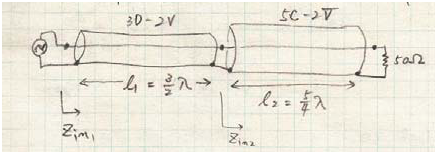
\includegraphics[width=140mm]{circuit.png}
    \caption{回路図}
    \label{p3}
  \end{center}
\end{figure}

周波数特性のグラフを出力するプログラムをソースコード \ref{sc1}に示す.

\lstinputlisting[caption=周波数特性,label=sc1]{/home/sofue/lab/py/transferFunction.py}

\newpage

ソースコード \ref{sc1} によって得られた周波数特性を図 \ref{p4} に示す.
図 \ref{p4}ではγの計算に, G = 0, Rは図 \ref{p1}, 図 \ref{p2}の導体抵抗[20℃]の値を使用している.


\begin{figure}[H]
  \begin{center}
    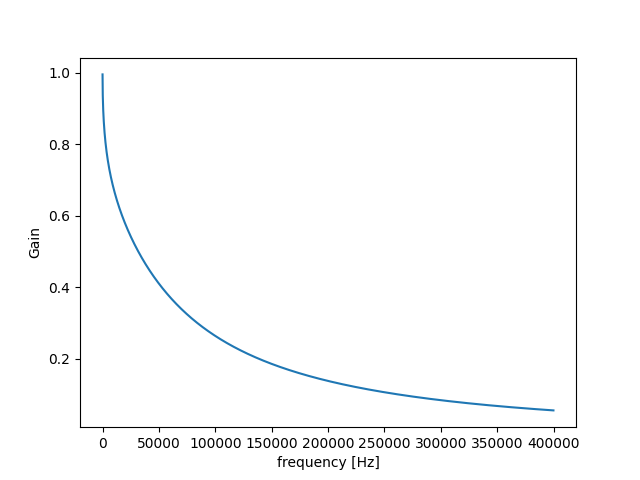
\includegraphics[width=140mm]{frequency_characteristic.png}
    \caption{周波数特性}
    \label{p4}
  \end{center}
\end{figure}

\begin{figure}[H]
  \begin{center}
    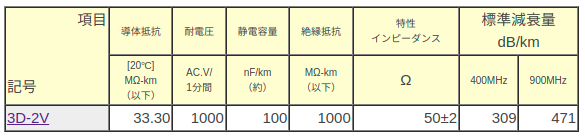
\includegraphics[width=140mm]{3d2v.png}
    \caption{3D-2Vケーブルの仕様}
    \label{p1}
  \end{center}
\end{figure}

\begin{figure}[H]
  \begin{center}
    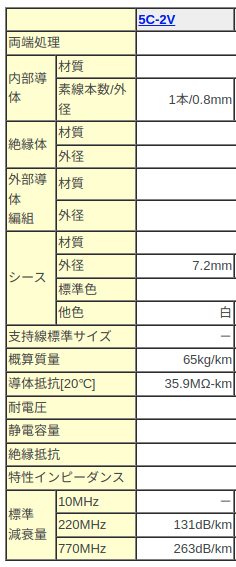
\includegraphics[width=70mm]{5c2v.png}
    \caption{5C-2Vケーブルの仕様}
    \label{p2}
  \end{center}
\end{figure}

また, R = 0, G = 0でγを計算した際の周波数特性を図 \ref{p5} に示す.

\begin{figure}[H]
  \begin{center}
    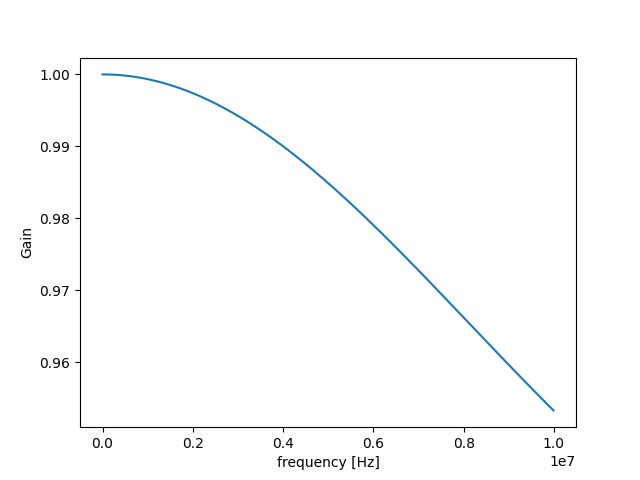
\includegraphics[width=150mm]{frequency_characteristic_lossless.png}
    \caption{無損失線路の周波数特性}
    \label{p5}
  \end{center}
\end{figure}

\section{おわりに}

今回は, 分布定数線路の周波数特性のグラフの縦軸を修正した.

\begin{thebibliography}{5}
  \bibitem{1}都築,”2020Q4-応用通信工学II-都築”, moodle内,参照 December 8,2021.
  \bibitem{2}システムギアダイレクト,"3D-2V無線用同軸ケーブル", https://www.systemgear.jp/kantsu/3d2v.php,参照 December 8,2021.
  \bibitem{3}システムギアダイレクト,”5C-2V同軸ケーブル”, https://www.systemgear.jp/kantsu/5c2v.php,参照 December 8,2021.
\end{thebibliography}

\end{document}